\documentclass[9pt, t]{beamer}
\usefonttheme{serif}
\usecolortheme[named=black]{structure}
\setbeamertemplate{footline}[frame number]{}
\setbeamertemplate{navigation symbols}{}

\usepackage[normalem]{ulem} % underlining
\setlength{\parskip}{0.5em}
\usepackage{tabto}
\renewcommand{\indent}{\hspace*{2em}}
% LANGUAGE + FONT
		    
\usepackage[english]{babel}

\usepackage{natbib}
\bibpunct[: ]{[}{]}{;}{a}{}{,}
\bibliographystyle{rusnat}

\usepackage{fontspec}  
\setmainfont{Fira Sans Book}


% DRAWING

\usepackage{tikz}
\usepackage{tikz-qtree}
\usetikzlibrary{shapes.geometric}
\usetikzlibrary{trees,arrows}
\usetikzlibrary{positioning}

% LINGUISTICS 

\usepackage{expex}
\lingset{aboveglftskip=0ex, belowglpreambleskip=0ex, belowexskip=1ex, aboveexskip=1ex, interpartskip=1ex}

\gathertags
\usepackage[glossaries]{leipzig}
% \makeglossaries

\usepackage{stmaryrd}

\usepackage[linguistics]{forest}

% MATH
\usepackage{amssymb}

\AtBeginSubsection[]
{
    \begin{frame}
        \frametitle{Table of Contents}
        \tableofcontents[currentsection,currentsubsection]
    \end{frame}
}

\resetcountonoverlays{excnt}

\title{вы зачем диахронически тривиальные вещи\\на структуру натягиваете?}
\subtitle{Andersson 2018. (*)ABA in Germanic verbs}
\author{аркадий шалдов}
\date{15.11.23, отв ридингруппа}

% -------------------------- текстиктекстиктекстик -----------------------------
\begin{document}

\NumTabs{14}

\begin{frame}
    \titlepage
\end{frame}

\begin{frame}
    \frametitle{*ABA что такое}

    В парадигмах ЕЯ элементы можно расположить так, чтобы среди множества форм ни одной лексемы не образовалось дыр
    
    \begin{itemize}
        \item[] где дыра — несинкретичная форма между двумя синкретичными формами
    \end{itemize}

    \only<1>{[Bobaljik 2012]

    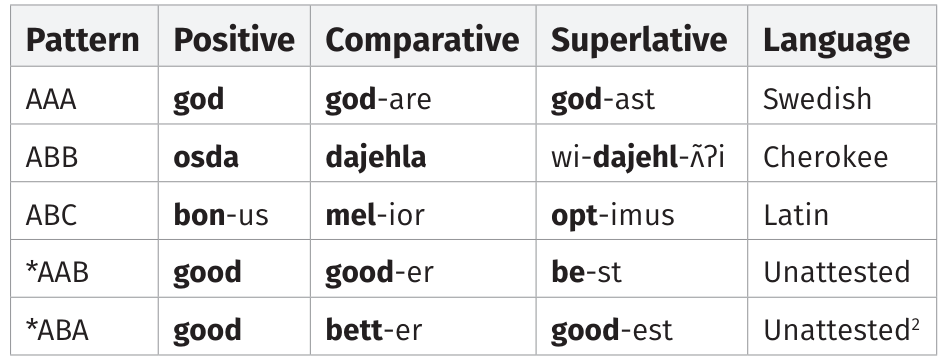
\includegraphics[width=30em]{images/adj.png}}

    \only<2>{
        Очень точное наблюдение [Bobaljik, Sauerland 2018]: 
        
        \begin{itemize}
            \item падежные маркеры
            \item число и падеж местоимений
            \item клюзивность местоимений
            \item дейктические выражения
            \item ...
            \item германские глаголы
        \end{itemize}
    }

\end{frame}

\begin{frame}
    \frametitle{Почему *ABA?}

    Как объяснить, что если значение X и значение Z выражаются одинаково, значение Y не выражается иначе?

    \begin{itemize}
        \item Bobaljik 2012: признаки вкладываются в определенном порядке: \textsc{[[[X] Y] Z]}
    
        \item Caha 2017: признаки оверлапятся: Y — это \textsc{[Z [X]]}
        
        \item Kramer 2015: X — это [+F], Y — это [], Z — это [-F]
        
        \item Graf 2017: трансдукции между графами!!!
    
    \end{itemize}
\end{frame}

\begin{frame}
    \frametitle{Почему не *ABA?}

    Иногда *ABA нарушается. Почему?
    
    \begin{itemize}
        \item У нас неверные посылки касательно парадигмы
        \pause

        \item Фонологические процессы создают видимость (отсутствия) синкретизма [Kasenov 2022]
        
        \pause
        \item Это просто совпадение двух несвязанных форм

        \begin{tabular}{r l}
            nom. &  окн-о\\
            gen. &  окн-а\\
            ins. &  окн-о-м\\
        \end{tabular}

        \pause 
        \item Нет здесь никакого *ABA
    \end{itemize}

\end{frame}

\begin{frame}
    \frametitle{К делу}

    Германские абляуты в глагольной парадигме наблюдают крепенькое *ABA, если расположить ее в порядке \textsc{present} > \textsc{participle} > \textsc{past} [Wiese 2008]

    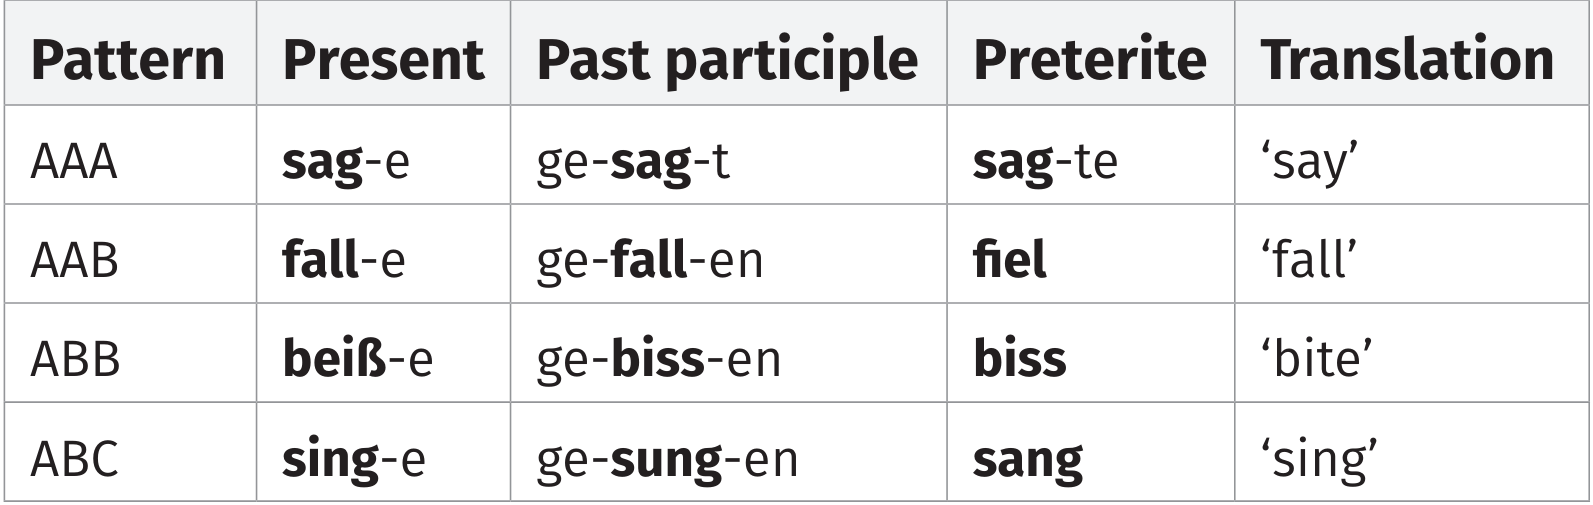
\includegraphics[width=25em]{images/german proper.png}
    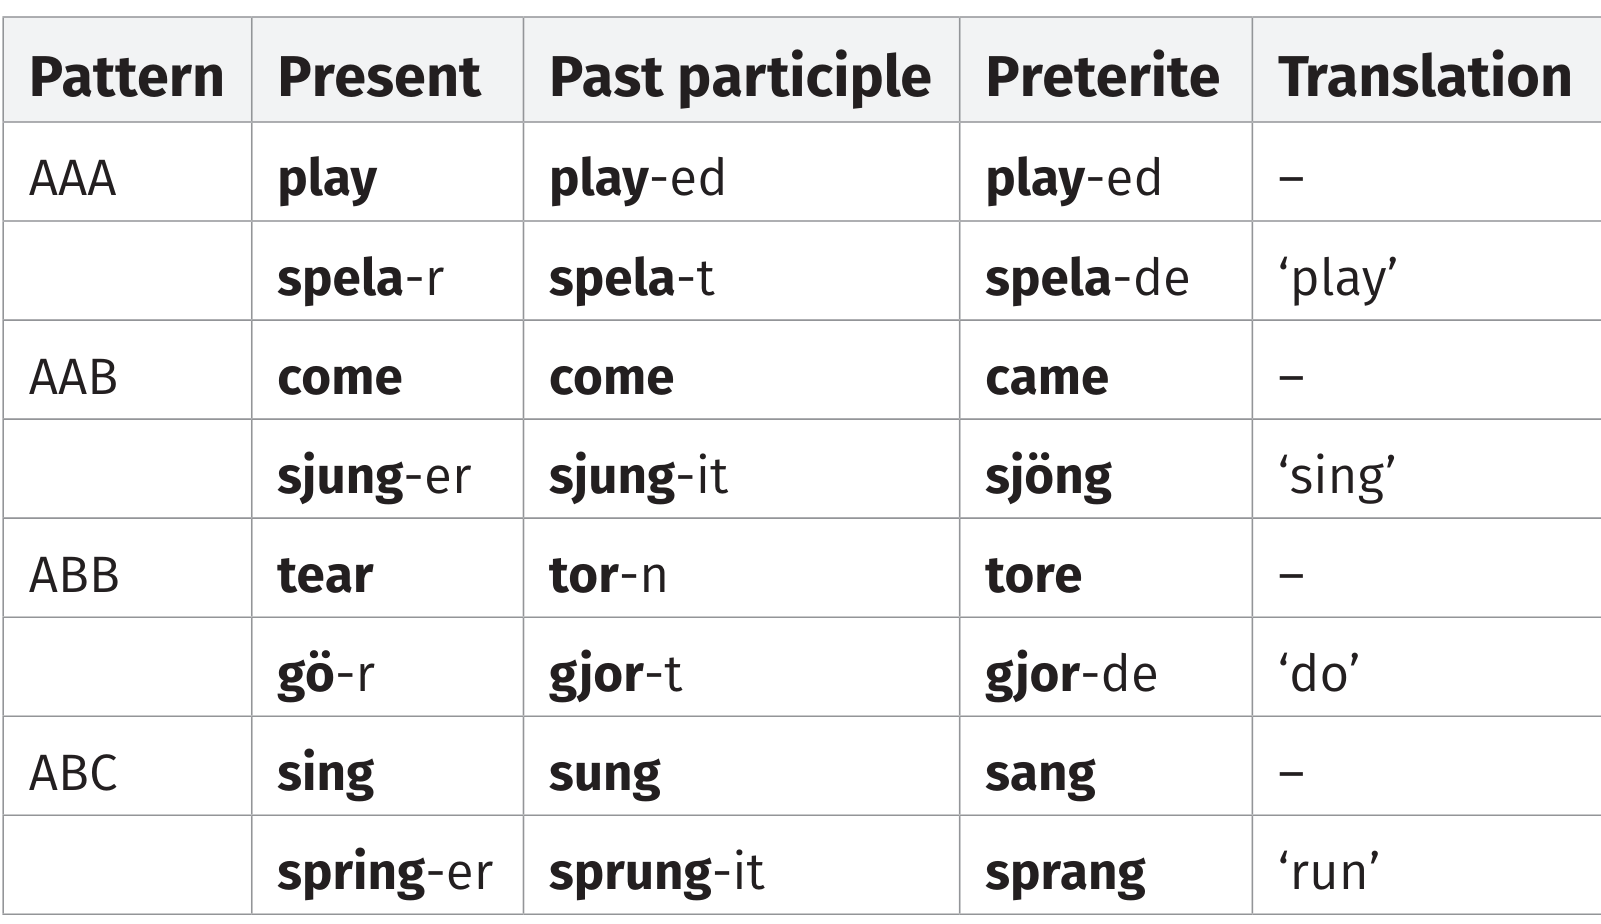
\includegraphics[width=25em]{images/english proper.png}

\end{frame}

\begin{frame}
    \frametitle{Как бы ABA}

    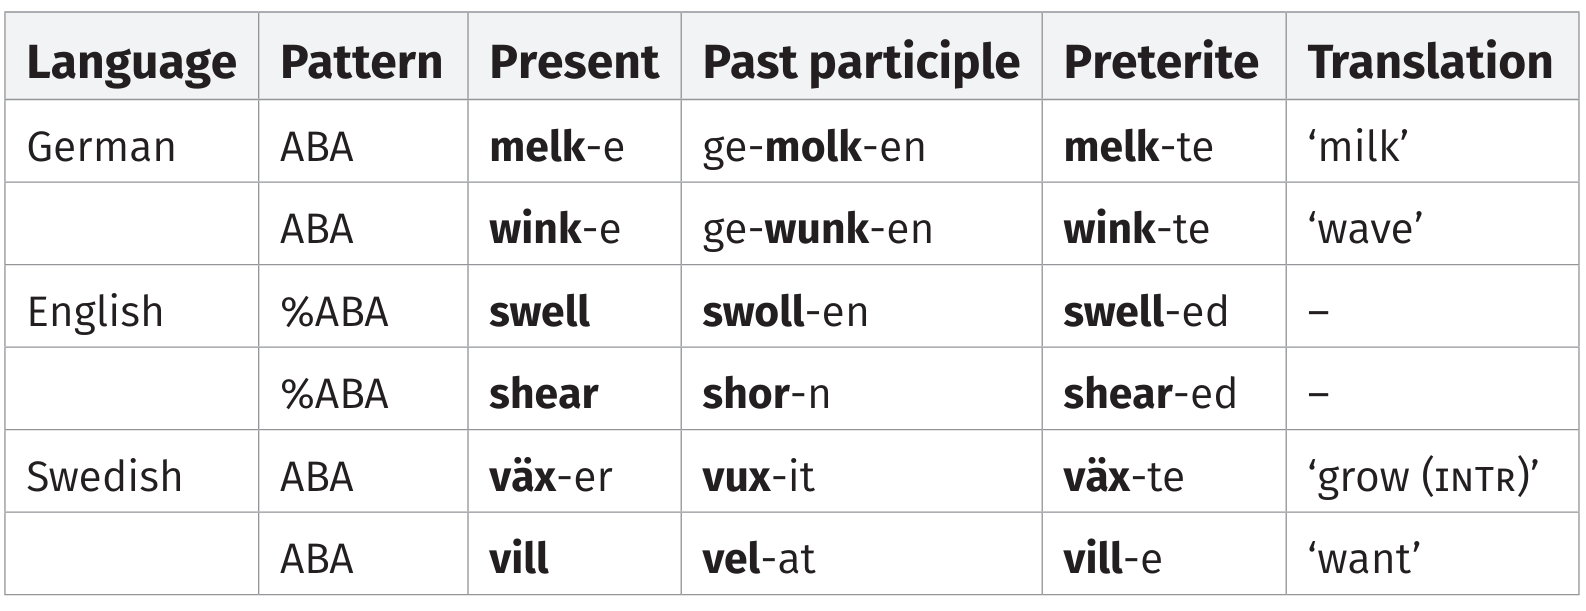
\includegraphics[width=25em]{images/not aba.png}

    Это разные «спряжения»: «слабое» и «сильное». Можно нашаманить (напр. добавить признаки \textsc{weak} и \textsc{strong}) и объяснить. Такое нам не интересно.

\end{frame}

\begin{frame}
    \frametitle{Реально ABA}

    \begin{enumerate}
        \item Шведский: в третье спряжение входит ABA-глагол 'иметь'
        
        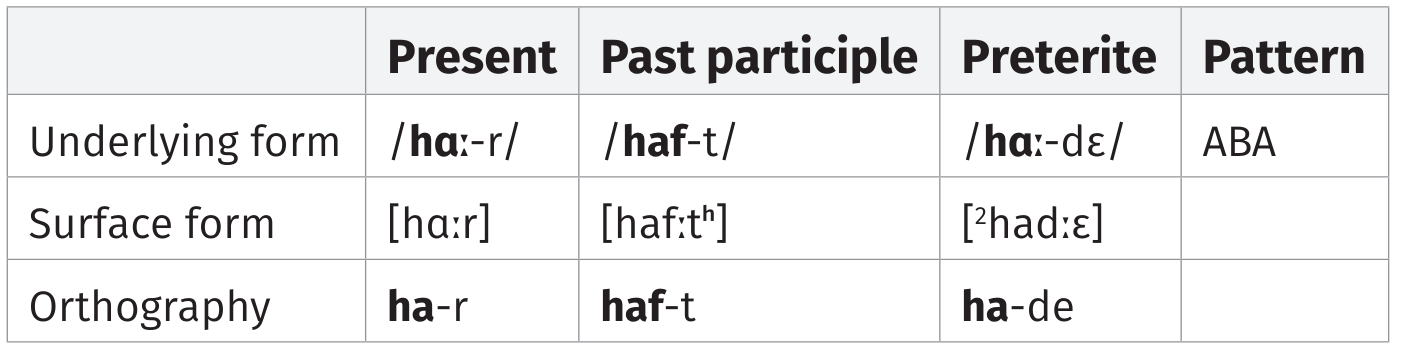
\includegraphics[width=25em]{images/har.png}

        \pause
        \item Нижненемецкий: глагол 'брать' (в ст. немецком /e:/-/o/-/a:/)
        
        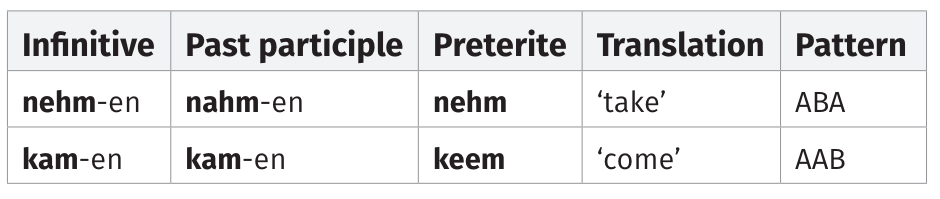
\includegraphics[width=25em]{images/nehmen.png}

        \pause
        \item Старошведский: 'спать' (и, возможно, целое спряжение!)
        
        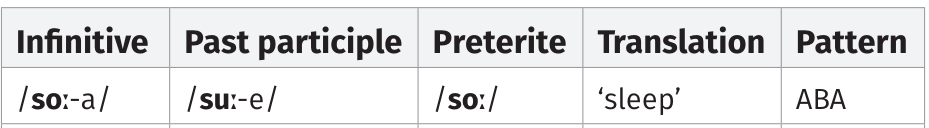
\includegraphics[width=25em]{images/sue.png}

    \end{enumerate}
\end{frame}
    
\begin{frame}
    \frametitle{Давайте объяснять диахронически!}

    Что если нет никакого баяса против ABA-паттернов?

    \begin{itemize}
        \item Просто в прагерманском был продуктивный абляут, и в нем не было ABA.
        
        \only<1>{
            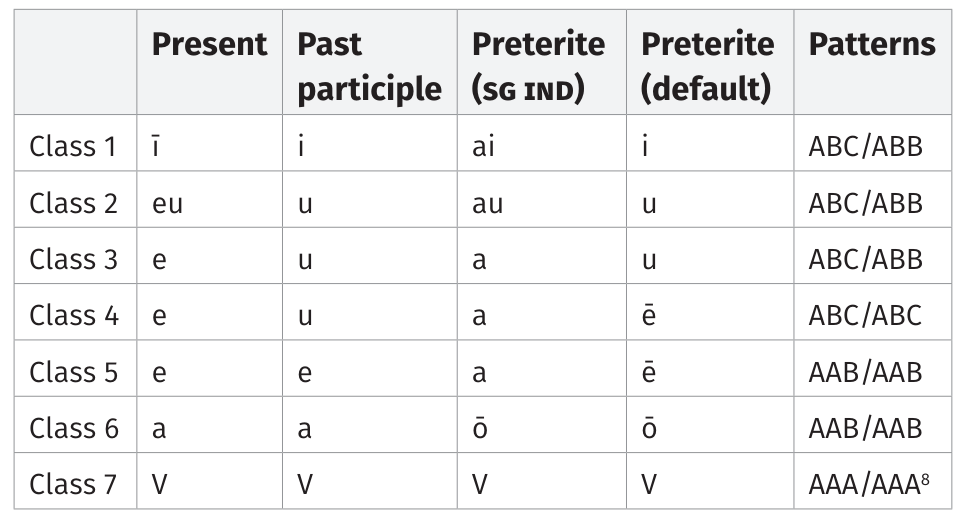
\includegraphics[width=25em]{images/proto.png}
        }

        \only<2->{
            \item Так уж вышло, что третья ступень абляута почти нигде не совпала с первой
        \end{itemize}
       
        $\Rightarrow$ *ABA в глагольных основах — не типологическое обобщение, а особенность одного языка
        \begin{itemize}
            \item которую, небось, тоже можно объяснить диахронически
        }
    \end{itemize}
\end{frame}

\begin{frame}
    \frametitle{Так уж вышло, что третья ступень абляута почти нигде не совпала с первой}

    Что значит \textit{так уж вышло}?!

    \begin{itemize}
        \item У нерегулярных парадигм два пути: сохраниться или выровняться [Lieberman et al. 2007]
        \pause

        \item Если парадигма выравнивается, становится AAA
        \item Если парадигма не выравнивается, остается AAB / ABB / ABC
        
        \pause
        \item Но все-таки изредка одна из ячеек парадигмы претерпивает изменения, а другая нет
        \begin{itemize}
            \item Это — вышеупомянутые случаи с разными спряжениями
        \end{itemize}
    \end{itemize}
\end{frame}

\begin{frame}[c]
    \frametitle{А знаете, с какими словами чаще всего происходят спорадические изменения?}

    \pause
    С частотными!

    Например, шведский глагол 'иметь' очень частотный, и с ним произошли спорадические изменения, и он стал ABA

\end{frame}

\begin{frame}
    \frametitle{Неспорадическое ABA}

    \begin{itemize}
        \item Но ведь разные гласные изменяются по-разному
        \pause
        \item Каков шанс, что гласные на двух концах парадигмы совпадут?
        \pause
        \item Например, очень высок для класса 6 (и очень низок для класса 4)
    \end{itemize}
    
    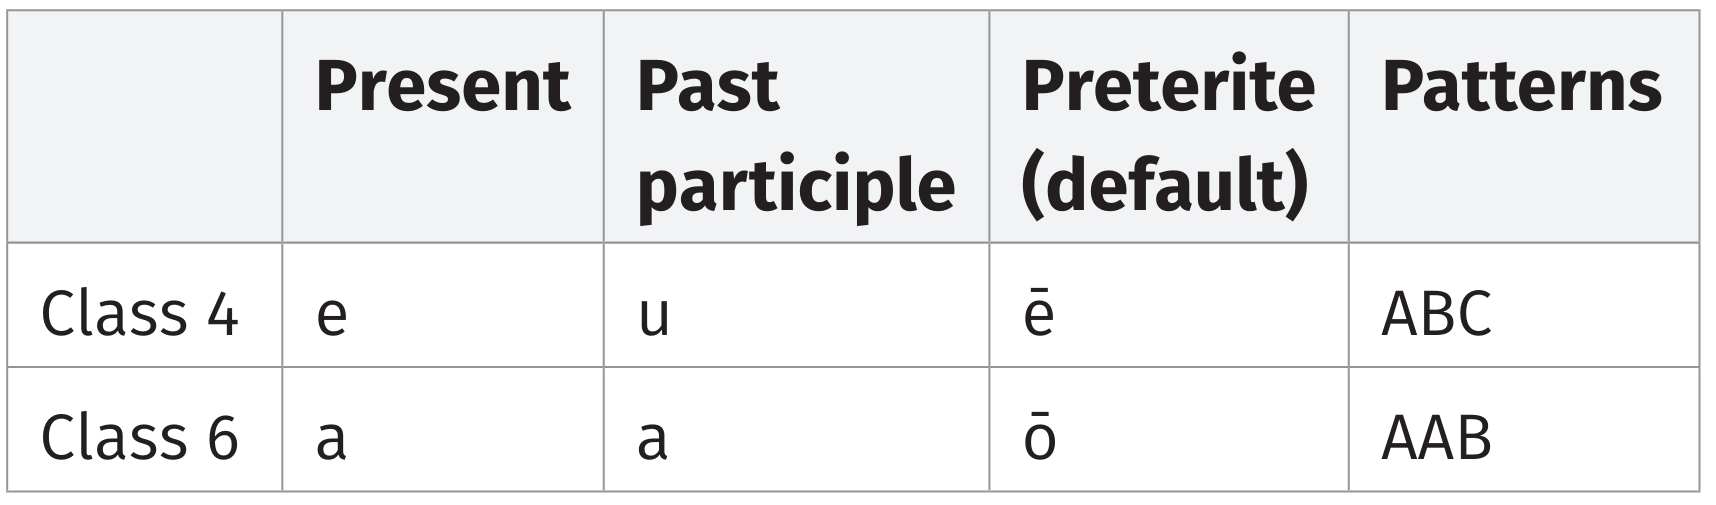
\includegraphics[width=20em]{images/two classes.png}
    
    \pause
    Кажется, именно это недавно произошло в старошведском

\end{frame}

\begin{frame}
    \frametitle{Неспорадическое ABA в старошведском}

    \only<1>{
        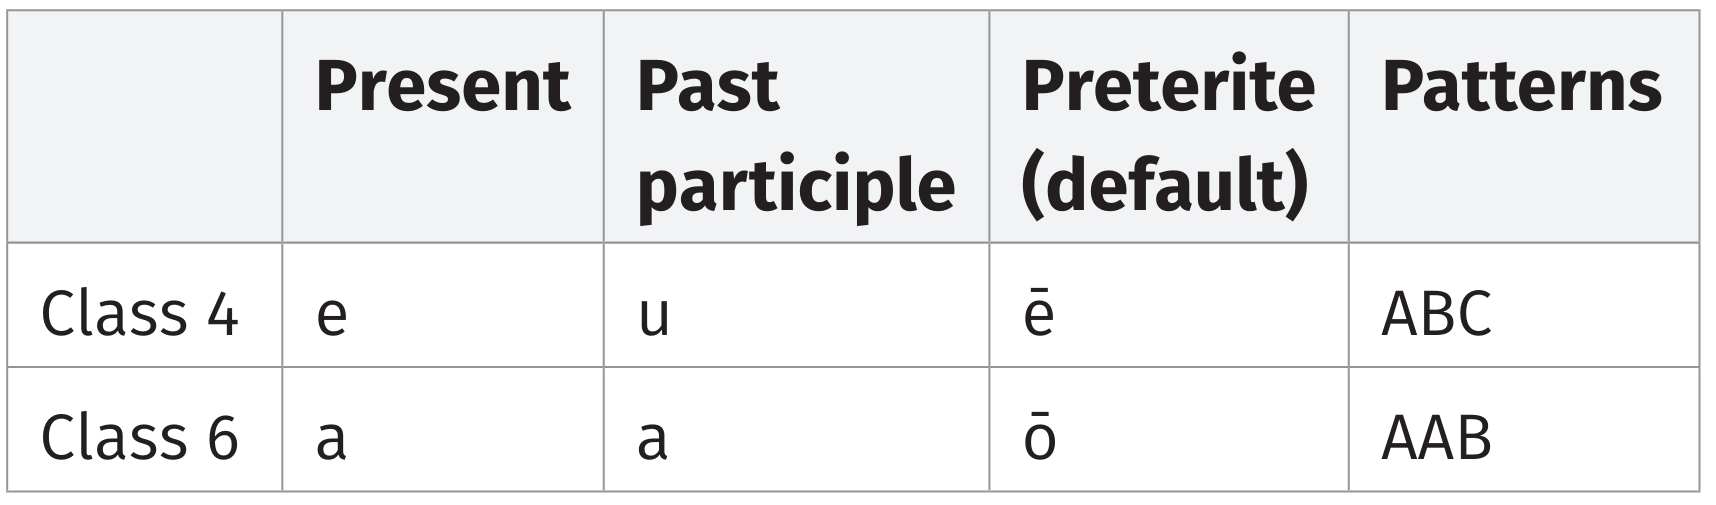
\includegraphics[width=20em]{images/two classes.png}
    }

    в 19 веке:

    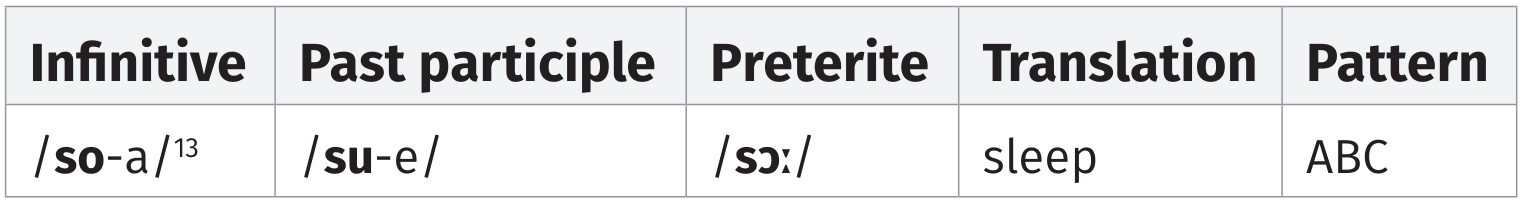
\includegraphics[width=25em]{images/19 cent.png}

    \pause
    
    а потом две o нейтрализовались

    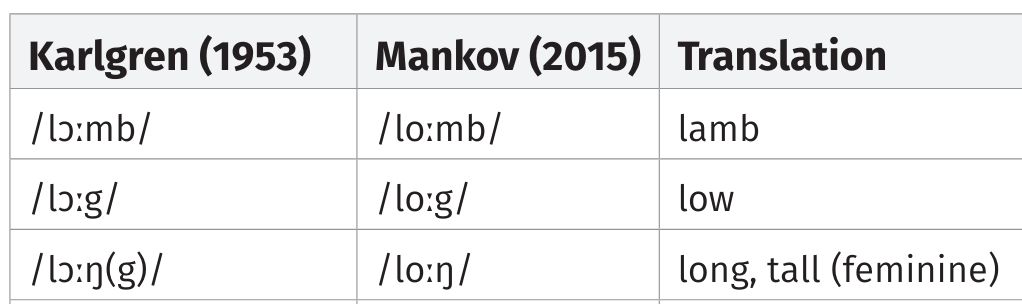
\includegraphics[width=20em]{images/change.png}

    и получилось

    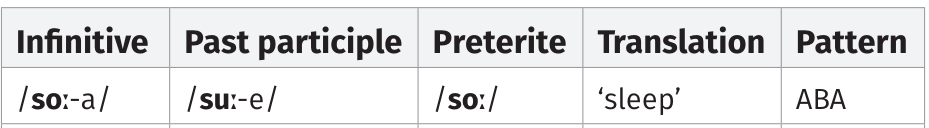
\includegraphics[width=20em]{images/sue.png}

    Вероятно, такое же ABA и в других глаголов 4 спряжения — мы не знаем

\end{frame}

\begin{frame}
    \frametitle{Как подтвердить?}

    Надо смотреть на другие языки

    \begin{enumerate}
        \item берем любой язык с алломорфией в трех и более глагольных формах
        \item ранжируем их, чтобы минимизировать ABA
        \item считаем исключения
    \end{enumerate}

    Есть исключения? Значит, надо объяснять как-нибудь еще.
\end{frame}

\begin{frame}
    \frametitle{Мораль}

    Можно ли объяснять ABA \textit{экстралингвистически}?
    \begin{itemize}
        \item С помощью диахронии — можно
        \item Функционально?
        \item Через освоение языка?
        \item Как-нибудь еще?
    \end{itemize}
    Похоже, занавес между формалистами и остальными людьми скрыл от последних наблюдения Бобалика и коллег
    
    Иначе как объяснить, что ни одно *ABA на момент написания статьи, видимо, не получило альтернативного объяснения?
    
\end{frame}

\end{document}